\begin{figure}[ht]
	\tikzsetnextfilename{plot_integral_riemannintegral}
	\begin{center}
		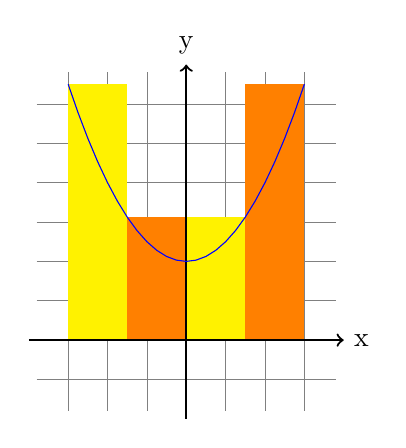
\begin{tikzpicture}
			\draw[very thin, gray, step = 0.5] (-1.9,-0.9) grid (1.9,3.4);
			\fill[yellow](-1.5,0) rectangle (-0.75,3.25);
			\fill[orange](-0.75,0) rectangle (0,1.56);
			\fill[yellow](0,0) rectangle (0.75, 1.56);
			\fill[orange](0.75,0) rectangle (1.5,3.25);
			\draw[->,thick, black](-2,0) -- (2,0) node[right]{x};
			\draw[->,thick, black](0,-1) -- (0,3.5) node[above]{y};
			\draw[blue, domain = -1.5 :1.5]  
				plot(\x, \x * \x + 1);
		\end{tikzpicture}
	\end{center}
	\caption{oberes Riemann-Integral}
	\label{fig_int_riemann}
\end{figure}